\documentclass[../main.tex]{subfiles}

\usepackage{makecell}
\usepackage{amsmath}

\titleformat{\section}
  {\normalsize\bfseries}{\thesection}{1em}{\normalfont}

\pagestyle{empty}

\setcounter{chapter}{7}
\pagenumbering{arabic}
\setcounter{page}{7}

\newenvironment{blockquote}{%
  \par%
  \medskip
  \leftskip=3.5em\rightskip=2em%
  \noindent\ignorespaces}{%
  \par\medskip}


\begin{document}

\chapter{}
\label{cha:cha_8}


\section{}
The flop counts for the tridiagonal algorithm in Fig. $8.6$ can be summarized as
\bigbreak
\begin{tabular}{|l|c|c|c|}
\hline
 &\textbf{ Mult/Div} &\textbf{ Add/Subtr} &\textbf{ Total} \\
\hline
\textbf{Forward elimination} & $3(n-1)$ & $2(n-1)$ & $5(n-1)$ \\
\hline
\textbf{Back substitution} & $2 n-1$ & $n-1$ & $3 n-2$ \\
\hline
\textbf{Total} & $5 n-4$ & $3 n-3$ & $\textbf{8 n-7}$ \\
\hline
\end{tabular}
\bigbreak
Thus, as $n$ increases, the effort is much, much less than for a full matrix solved with Gauss elimination which is proportional to $n^{3}$.
\bigbreak


\section{}
The equations can be expressed in a format that is compatible with graphing $x_{2}$ versus $x_{1}$ :
\bigbreak$
\begin{aligned}
&x_{2}=0.5 x_{1}+3 \\\\
&x_{2}=-\dfrac{1}{6} x_{1}+\dfrac{34}{6}
\end{aligned}$
\bigbreak
which can be plotted as
\bigbreak
\begin{figure}[H]
		\hspace*{1.5cm}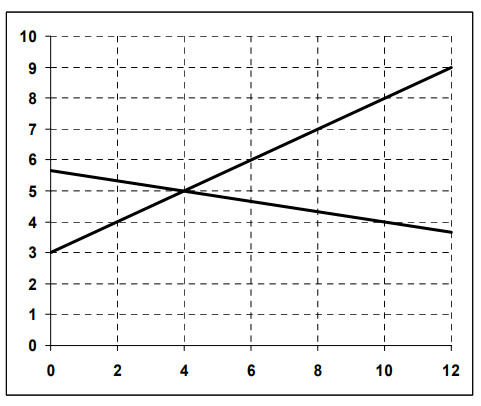
\includegraphics[width=0.5\linewidth]{fig_8_1}
		\label{fig:fig_8_1}
	\end{figure}
	

\bigbreak
Thus, the solution is $x_{1}=4, x_{2}=5$. The solution can be checked by substituting it back into the equations to give
\bigbreak
$4(4)-8(5)=16-40=-24$
\bigbreak
$4+6(5)=4+30=34$
\bigbreak


\section{}
\begin{enumerate}[label=\bfseries(\alph*)]
\item The equations can be expressed in a format that is compatible with graphing $x_{2}$ versus $x_{1}$ :
\bigbreak$
\begin{aligned}
&x_{2}=0.11 x_{1}+12 \\
&x_{2}=0.114943 x_{1}+10
\end{aligned}$
\bigbreak
which can be plotted as
\bigbreak
\begin{figure}[H]
		\hspace*{1cm}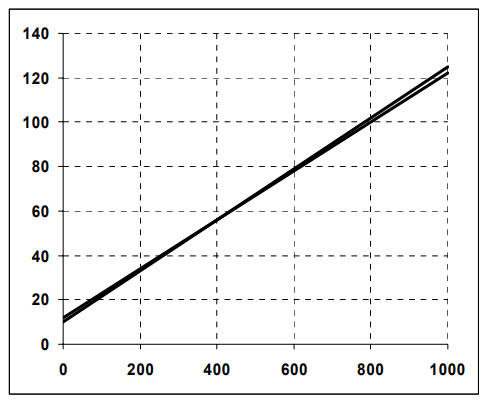
\includegraphics[width=0.5\linewidth]{fig_8_2}
		\label{fig:fig_8_2}
	\end{figure}
	\bigbreak
	
Thus, the solution is approximately $x_{1}=400, x_{2}=60$. The solution can be checked by substituting it back into the equations to give
\bigbreak$
\begin{aligned}
&-1.1(400)+10(60)=160 \approx 120 \\
&-2(400)+17.4(60)=244 \approx 174
\end{aligned}$
\bigbreak
Therefore, the graphical solution is not very good.
\bigbreak
\item Because the lines have very similar slopes, you would expect that the system would be ill-conditioned
\bigbreak
\item The determinant can be computed as
\bigbreak
$\left|\begin{array}{cc}
-1.1 & 10 \\
-2 & 17.4
\end{array}\right|=-1.1(17.2)-10(-2)=-19.14+20=0.86$
\bigbreak
This result is relatively low suggesting that the solution is ill-conditioned.
\bigbreak
\end{enumerate}

\section{}
\begin{enumerate}[label=\bfseries(\alph*)]
\item he determinant can be evaluated as
\bigbreak$
\begin{aligned}
&D=0\left[\begin{array}{cc}
2 & -1 \\
-2 & 0
\end{array}\right]-(-3)\left[\begin{array}{cc}
1 & -1 \\
5 & 0
\end{array}\right]+7\left[\begin{array}{cc}
1 & 2 \\
5 & -2
\end{array}\right] \\\\
&D=0(-2)+3(5)+7(-12)=-69
\end{aligned}$
\bigbreak
\item Cramer's rule 
\bigbreak$
\begin{aligned}
& x_{1}=\dfrac{\left|\begin{array}{ccc}2 & -3 & 7 \\3 & 2 & -1 \\2 & -2 & 0\end{array}\right|}{-69}=\dfrac{-68}{-69}=0.9855 \\\\
& x_{2}=\dfrac{\left|\begin{array}{ccc}0 & 2 & 7 \\1 & 3 & -1 \\5 & 2 & 0\end{array}\right|}{-69}=\dfrac{-101}{-69}=1.4638 \\\\
& x_{3}=\dfrac{\left|\begin{array}{ccc}0 & -3 & 2 \\1 & 2 & 3 \\5 & -2 & 2\end{array}\right|}{-69}=\dfrac{-63}{-69}=0.9130 
\end{aligned}$
\bigbreak

\item Pivoting is necessary, so switch the first and third rows,
\bigbreak$
\begin{aligned}
5 x_{1}-2 x_{2}& \quad\quad=2 \\
x_{1}+2 x_{2}&-x_{3}=3 \\
-3 x_{2}&+7 x_{3}=2
\end{aligned}$
\bigbreak
Multiply pivot row 1 by $1 / 5$ and subtract the result from the second row to eliminate the $a_{21}$ term.
\bigbreak$
\begin{aligned}
5 x_{1}-2 x_{2}& \quad\quad=2 \\
2.4 x_{2}&-x_{3}=2.6 \\
-3 x_{2}&+7 x_{3}=2
\end{aligned}$
\bigbreak
Pivoting is necessary so switch the second and third row,
\bigbreak$
\begin{aligned}
5 x_{1}-2 x_{2}		&	\quad\quad		=2 \\
-3 x_{2}&+7 x_{3}=2 \\
2.4 x_{2}&-x_{3}=2.6
\end{aligned}$
\bigbreak
Multiply pivot row 2 by $2.4 /(-3)$ and subtract the result from the third row to eliminate the $a_{32}$ term.
\bigbreak$
\begin{aligned}
5 x_{1}		&-2 x_{2}	&&=2 \\
				&-3 x_{2}		&+7 x_{3}&=2 \\
& &4.6 x_{3}&=4.2
\end{aligned}$
\bigbreak
The solution can then be obtained by back substitution
\bigbreak$
\begin{aligned}
&x_{3}=\dfrac{4.2}{4.6}=0.913043 \\\\
&x_{2}=\dfrac{2-7(0.913043)}{-3}=1.463768\\\\
&x_{1}=\dfrac{2+2(1.463768)}{5}=0.985507
\end{aligned}$
\bigbreak
\bigbreak
\item
$-3(1.463768)+7(0.913043)=2$
\bigbreak
$0.985507+2(1.463768)-(0.913043)=3$
\bigbreak
$5(0.985507)-2(1.463768)=2$
\bigbreak

\section{}
\underline{Prob. 8.3:}
\bigbreak
\begin{lstlisting}[numbers=none]
>> A=[-1.1 10;-2 17.4];
>> det(A)

ans =
	  0.8600
\end{lstlisting}
\bigbreak
\underline{Prob. 8.4:}
\bigbreak
\begin{lstlisting}[numbers=none]
>> A=[0 -3 7;1 2 -1;5 -2 0];
>> det(A)

ans =
 	 -69 

\bigbreak
\end{lstlisting}
\end{enumerate}


\section{}
\begin{enumerate}[label=\bfseries(\alph*)]
\item The equations can be expressed in a format that is compatible with graphing $x_{2}$ versus $x_{1}$ :
\bigbreak

$x_{2}=0.5 x_{1}+9.5$
\bigbreak
$x_{2}=0.51 x_{1}+9.4$
\bigbreak
The resulting plot indicates that the intersection of the lines is difficult to detect:
\bigbreak
\begin{figure}[H]
		\hspace*{0.7cm}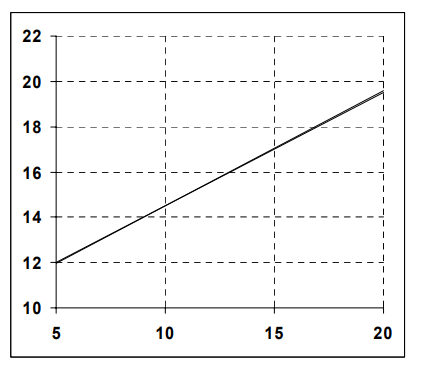
\includegraphics[width=0.5\linewidth]{fig_8_3}
		\label{fig:fig_8_3}
	\end{figure}
	\bigbreak

Only when the plot is zoomed is it at all possible to discern that solution seems to lie at about $x_{1}=14.5$ and $x_{2}=10$.
\bigbreak
\begin{figure}[H]
		\hspace*{0.7cm}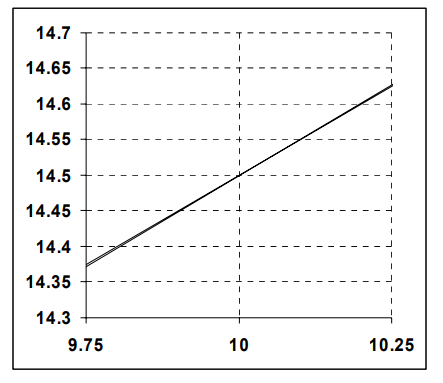
\includegraphics[width=0.5\linewidth]{fig_8_4}
		\label{fig:fig_8_4}
	\end{figure}
	\bigbreak

\item The determinant can be computed as
\bigbreak
$\left|\begin{array}{cc}0.5 & -1 \\ 1.02 & -2\end{array}\right|=0.5(-2)-(-1)(1.02)=0.02$
\bigbreak
which is close to zero.
\bigbreak

\item Because the lines have very similar slopes and the determinant is so small, you would expect that the system would be ill-conditioned
\bigbreak
\item Multiply the first equation by $1.02 / 0.5$ and subtract the result from the second equation to eliminate the $x_{1}$ term from the second equation,
\bigbreak
$
\begin{aligned}
0.5 x_{1}-x_{2}=-9.5 \\
0.04 x_{2}=0.58
\end{aligned}$
\bigbreak
The second equation can be solved for
\bigbreak
$x_{2}=\dfrac{0.58}{0.04}=14.5$
\bigbreak
This result can be substituted into the first equation which can be solved for
\bigbreak
$x_{1}=\dfrac{-9.5+14.5}{0.5}=10$
\bigbreak

\item Multiply the first equation by $1.02 / 0.52$ and subtract the result from the second equation to eliminate the $x_{1}$ term from the second equation,
\bigbreak
$
\begin{aligned}
0.52 x_{1}&\quad\quad\quad-x_{2}=-9.5 \\&
-0.03846 x_{2}=-0.16538
\end{aligned}$
\bigbreak
The second equation can be solved for
\bigbreak
$x_{2}=\dfrac{-0.16538}{-0.03846}=4.3$
\bigbreak
This result can be substituted into the first equation which can be solved for
\bigbreak
$x_{1}=\dfrac{-9.5+4.3}{0.52}=-10$
\bigbreak
Interpretation: The fact that a slight change in one of the coefficients results in a radically different solution illustrates that this system is very ill-conditioned.
\bigbreak
\end{enumerate}

\section{}
\begin{enumerate}[label=\bfseries(\alph*)]
\item Multiply the first equation by $-3 / 10$ and subtract the result from the second equation to eliminate the $x_{1}$ term from the second equation. Then, multiply the first equation by $1 / 10$ and subtract the result from the third equation to eliminate the $x_{1}$ term from the third equation.
\bigbreak$
\begin{aligned}
10 x_{1}+2 x_{2} \quad-x_{3} &=27 \\
-5.4 x_{2}+1.7 x_{3} &=-53.4 \\
0.8 x_{2}+5.1 x_{3} &=-24.2
\end{aligned}$
\bigbreak
Multiply the second equation by $0.8 /(-5.4)$ and subtract the result from the third equation to eliminate the $x_{2}$ term from the third equation,
\bigbreak$
\begin{aligned}
10 x_{1}+2 x_{2} \quad&-x_{3}\quad\quad=27 \\
-5.4 x_{2} \quad&+1.7 x_{3}\quad=-53.4 \\
&5.351852 x_{3}=-32.11111 
\end{aligned}$
\bigbreak
Back substitution can then be used to determine the unknowns
\bigbreak$
\begin{aligned}
&x_{3}=\dfrac{-32.11111}{5.351852}=-6 \\\\
&x_{2}=\dfrac{(-53.4-1.7(-6))}{-5.4}=8 \\\\
&x_{1}=\dfrac{(27-6-2(8))}{10}=0.5
\end{aligned}$
\bigbreak
\item Check:
\bigbreak$
\begin{aligned}
&10(0.5)+2(8)-(-6)=27 \\
&-3(0.5)-6(8)+2(-6)=-61.5 \\
&0.5+8+5(-6)=-21.5
\end{aligned}$
\bigbreak
\end{enumerate}

\section{}
\begin{enumerate}[label=\bfseries(\alph*)]
\item Pivoting is necessary, so switch the first and third rows,
\bigbreak$
\begin{aligned}
&-8 x_{1}+x_{2}-2 x_{3}=-20 \\
&-3 x_{1}-x_{2}+7 x_{3}=-34 \\
&2 x_{1}-6 x_{2}-x_{3}=-38
\end{aligned}$
\bigbreak
Multiply the first equation by $-3 /(-8)$ and subtract the result from the second equation to eliminate the $a_{21}$ term from the second equation. Then, multiply the first equation by $2 /(-8)$ and subtract the result from the third equation to eliminate the $a_{31}$ term from the third equation.
\bigbreak$
\begin{gathered}
-8 x_{1} \quad+x_{2} \quad-2 x_{3}=-20 \\
-1.375 x_{2}+7.75 x_{3}=-26.5 \\
-5.75 x_{2}-1.5 x_{3}=-43
\end{gathered}$
\bigbreak
Pivoting is necessary so switch the second and third row,
\bigbreak$
\begin{gathered}
-8 x_{1} \quad+x_{2} \quad-2 x_{3}=-20 \\
-5.75 x_{2}-1.5 x_{3} =-43 \\
-1.375 x_{2}+7.75 x_{3} =-26.5
\end{gathered}$
\bigbreak
Multiply pivot row 2 by $-1.375 /(-5.75)$ and subtract the result from the third row to eliminate the $a_{32}$ term.
\bigbreak$
\begin{aligned}
-8 x_{1}\quad+x_{2} \quad -2 x_{3}  &=-20 \\
\quad-5.75 x_{2}  -1.5 x_{3}  &=-43 \\
\quad8.108696 x_{3}  &=-16.21739
\end{aligned}$
\bigbreak
The solution can then be obtained by back substitution
\bigbreak$
\begin{aligned}
&x_{3}=\dfrac{-16.21739}{8.108696}=-2 \\\\
&x_{2}=\dfrac{-43+1.5(-2)}{-5.75}=8
\end{aligned}$
\bigbreak
$x_{1}=\dfrac{-20+2(-2)-1(8)}{-8}=4$
\bigbreak
\item Check:
\bigbreak$
\begin{aligned}
&2(4)-6(8)-(-2)=-38 \\
&-3(4)-(8)+7(-2)=-34 \\
&-8(4)+(8)-2(-2)=-20
\end{aligned}$
\bigbreak


\section{}
Multiply the first equation by $-0.4 / 0.8$ and subtract the result from the second equation to eliminate the $x_{1}$ term from the second equation.
\bigbreak
$\left[\begin{array}{ccc}
0.8 & -0.4 & \\
& 0.6 & -0.4 \\
& -0.4 & 0.8
\end{array}\right]\left\{\begin{array}{l}
x_{1} \\
x_{2} \\
x_{3}
\end{array}\right\}=\left\{\begin{array}{c}
41 \\
45.5 \\
105
\end{array}\right\}$
\bigbreak
Multiply pivot row 2 by $-0.4 / 0.6$ and subtract the result from the third row to eliminate the $x_{2}$ term.
\bigbreak
$\left[\begin{array}{ccc}
0.8 & -0.4 &\\
& 0.6 & -0.4 \\
& & 0.533333
\end{array}\right]\left\{\begin{array}{l}
x_{1} \\
x_{2} \\
x_{3}
\end{array}\right\}=\left\{\begin{array}{c}
41 \\
45.5 \\
135.3333
\end{array}\right\}$
\bigbreak
The solution can then be obtained by back substitution
\bigbreak$
\begin{aligned}
&x_{3}=\dfrac{135.3333}{0.533333}=253.75 \\\\
&x_{2}=\dfrac{45.5-(-0.4) 253.75}{0.6}=245 \\\\
&x_{1}=\dfrac{41-(-0.4) 245}{0.8}=173.75
\end{aligned}$
\bigbreak
\item Check:
\bigbreak$
\begin{aligned}
&0.8(173.75)-0.4(245)=41 \\
&-0.4(173.75)+0.8(245)-0.4(253.75)=25 \\
&-0.4(245)+0.8(253.75)=105
\end{aligned}$
\bigbreak


\section{}
The mass balances can be written as
\bigbreak$
\begin{aligned}
& Q_{21} c_{2}+400=Q_{12} c_{1}+Q_{13} c_{1} \\
& Q_{12} c_{1}=Q_{21} c_{2}+Q_{23} c_{2} \\
& Q_{13} c_{1}+Q_{23} c_{2}=Q_{33} c_{3}+200 \\\\
& \text { or collecting terms } \\\\
& \left(Q_{12}+Q_{13}\right) c_{1} \quad-Q_{21} c_{2} \quad&=400 \\
& -Q_{12} c_{1}+\left(Q_{21}+Q_{23}\right) c_{2}&=0 \\
& -Q_{13} c_{1} \quad-Q_{23} c_{2}\quad\quad+Q_{33} c_{3}&=200 
\end{aligned}$
\bigbreak
Substituting the values for the flows and expressing in matrix form
\bigbreak
$\left[\begin{array}{ccc}
120 & -20 & 0 \\
-80 & 80 & 0 \\
-40 & -60 & 120
\end{array}\right]\left\{\begin{array}{l}
c_{1} \\
c_{2} \\
c_{3}
\end{array}\right\}=\left\{\begin{array}{c}
400 \\
0 \\
200
\end{array}\right\}$
\bigbreak
A solution can be obtained with MATLAB as
\bigbreak
\begin{lstlisting}[numbers=none]
>> A = [120 -20 0;-80 80 0;-40 -60 120];
>> b = [400 0 200]';
>> c = a\b

c =
 	  4.0000
 	  4.0000
 	  5.0000

\end{lstlisting}
\bigbreak


\section{}
Equations for the amount of sand, fine gravel and coarse gravel can be written as
\bigbreak$
\begin{aligned}
&0.32 x_{1}+0.25 x_{2}+0.35 x_{3}=6000 \\
&0.30 x_{1}+0.40 x_{2}+0.15 x_{3}=5000 \\
&0.38 x_{1}+0.35 x_{2}+0.50 x_{3}=8000
\end{aligned}$
\bigbreak
where $x_{i}=$ the amount of gravel taken from pit $i$. MATLAB can be used to solve this system of equations for
\bigbreak
\begin{lstlisting}[numbers=none]
>> A=[0.32 0.25 0.35;0.3 0.4 0.15;0.38 0.35 0.5];
>> b=[6000;5000;8000];
>> x=A\b

x =
  1.0e+003 *
 	  7.0000
 	  4.4000
 	  7.6000
\end{lstlisting}
\bigbreak
Therefore, we take 7000,4400 and $7600 \mathrm{~m}^{3}$ from pits 1,2 and 3 respectively.
\bigbreak


\section{}
Substituting the parameter values the heat-balance equations can be written for the four nodes as
\bigbreak$
\begin{aligned}
&-40+2.2 T_{1}-T_{2}=4 \\
&-T_{1}+2.2 T_{2}-T_{3}=4 \\
&-T_{2}+2.2 T_{3}-T_{4}=4 \\
&-T_{3}+2.2 T_{4}-200=4
\end{aligned}$
\bigbreak
Collecting terms and expressing in matrix form
\bigbreak
$\left[\begin{array}{cccc}
2.2 & -1 & 0 & 0 \\
-1 & 2.2 & -1 & 0 \\
0 & -1 & 2.2 & -1 \\
0 & 0 & -1 & 2.2
\end{array}\right]\left\{\begin{array}{l}
T_{1} \\
T_{2} \\
T_{3} \\
T_{4}
\end{array}\right\}=\left\{\begin{array}{c}
44 \\
4 \\
4 \\
204
\end{array}\right\}$
\bigbreak
The solution can be obtained with MATLAB as
\bigbreak
\begin{lstlisting}[numbers=none]
>> A=[2.2 -1 0 0;-1 2.2 -1 0;0 -1 2.2 -1;0 0 -1 2.2]
>> b=[44 4 4 204]'
>> T=A\b

T =
 	 50.7866
 	 67.7306
	 94.2206
	 135.5548 
\end{lstlisting}

\end{enumerate}
\end{document}

